\documentclass{llncs}
\usepackage{times}
\usepackage[T1]{fontenc}
\usepackage[utf8]{inputenc}

% Comentar para not MAC Users
%\usepackage[applemac]{inputenc}

\usepackage{a4}
%\usepackage[margin=3cm,nohead]{geometry}
\usepackage{epstopdf}
\usepackage{graphicx}
\usepackage{fancyvrb}
\usepackage{amsmath}
\usepackage{subcaption}
\usepackage[bookmarks=false]{hyperref}
%\renewcommand{\baselinestretch}{1.5}

\begin{document}
\mainmatter
\title{TP4: Redes sem fios (802.11)}

\titlerunning{TP4: Redes sem fios (802.11)}

\author{Diogo Afonso Costa \and Daniel Maia \and Vitor Castro}

\authorrunning{Diogo Afonso Costa \and Daniel Maia \and Vitor Castro}

\institute{
University of Minho, Department of  Informatics, 4710-057 Braga, Portugal\\
e-mail: \{a78034,a77531,a77870\}@alunos.uminho.pt
}

\date{12 de dezembro de 2017}
\bibliographystyle{splncs}

\maketitle
\begin{abstract}

Este trabalho tem como objectivo explorar as particularidades do protocolo IEEE 802.11, especificamente, o formato das tramas, o endereçamento dos componentes envolvidos na comunicação sem fios e os tipos de tramas mais comuns, bem como a operação do protocolo.

\end{abstract}

\section{Introdução}



\clearpage
\section{Acesso Rádio (Para a trama correspondente 733)}

\subsection{Exercício 1}
\subsubsection{Questão}\rule[-10pt]{0pt}{10pt}\\

Identifique em que frequência do espectro está a operar a rede sem fios, e o canal que corresponde essa frequência.

\subsubsection{Resposta}\rule[-10pt]{0pt}{10pt}\\

A rede sem fios encontra-se a operar numa frequência de 2462MHz, que consequentemente pertence ao espectro dos 2GHz. 

Além disso, o canal usado é o número 11.

\subsubsection{Realização}\rule[-10pt]{0pt}{10pt}\\

\begin{figure}
  \begin{center}
  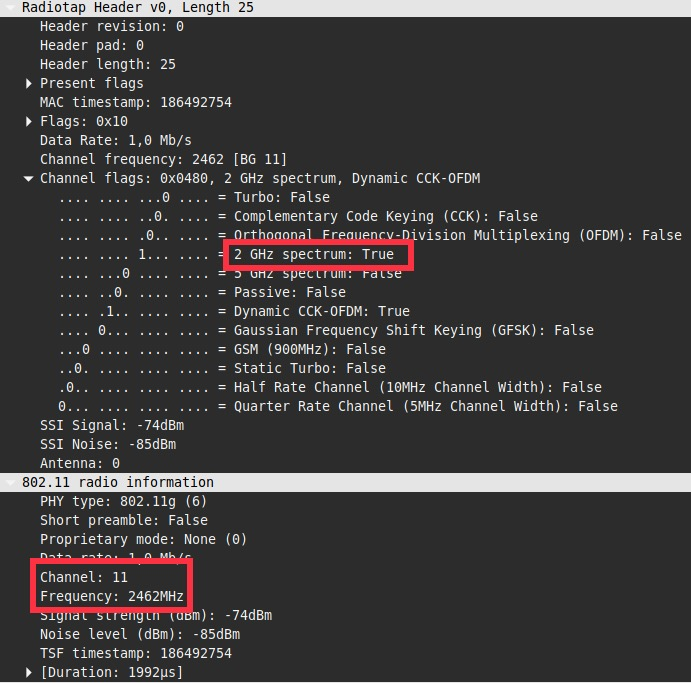
\includegraphics[scale=0.35]{./imagens/ex1.png} 
  \end{center}
  \caption{Frequência do espectro em que a rede sem fios se encontra a operar assim como o respetivo canal.}
  \label{fig:freq}
\end{figure}


\clearpage
\subsection{Exercício 2}
\subsubsection{Questão}\rule[-10pt]{0pt}{10pt}\\

Identifique a versão da norma IEEE 802.11 que está a ser usada.

\subsubsection{Resposta}\rule[-10pt]{0pt}{10pt}\\

A versão utilizada é a IEEE 802.11g.

\subsubsection{Realização}\rule[-10pt]{0pt}{10pt}\\

\begin{figure}
  \begin{center}
  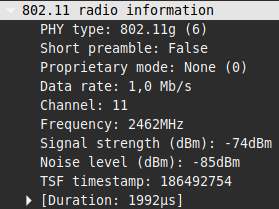
\includegraphics[scale=0.6]{./imagens/ex2.png} 
  \end{center}
  \caption{Versão da norma IEEE utilizada.}
  \label{fig:norma_ieee}
\end{figure}


\clearpage
\subsection{Exercício 3}
\subsubsection{Questão}\rule[-10pt]{0pt}{10pt}\\

Qual o débito a que foi enviada a trama escolhida? Será que esse débito corresponde ao débito máximo a que a interface WiFi pode operar? Justifique.

\subsubsection{Resposta}\rule[-10pt]{0pt}{10pt}\\

A trama escolhida foi enviada a 1.0 Mb/s. Visto tratar-se de uma trama que usa a norma IEEE 802.11g tem-se por defeito acesso a débitos até 54 Mb/s \cite{computer_networking}.

Efetivamente, a razão pela qual o débito se encontra consideravelmente baixo em relação ao máximo permitido pode resultar de diferentes fatores. Nomeadamente, quando a distância entre o \textit{host} e o ponto de acesso (AP) aumenta, o \textit{signal-to-noise ratio} (SNR) aumenta e o bit error ratio (BER) também. Por forma a combater o declinio na qualidade da ligação, caso a distância assim o justifique, o débito a que a trama é transmitida pode ser diminuido por forma a aumentar o SNR e o BER. Deste modo, também por esta razão a frequência que se encontra a operar a ligação seja relativamente baixa (2462 MHz) quando comparada com a frequência máxima que uma ligação 802.11g pode oferecer, ou seja, 5 GHz \cite{computer_networking} \cite{wiki:ber} \cite{wiki:snr}.

\subsubsection{Realização}\rule[-10pt]{0pt}{10pt}\\

\begin{figure}[h]
  \centering
  \begin{subfigure}{0.5\textwidth}
    \centering
    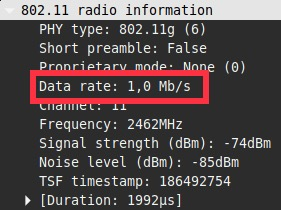
\includegraphics[width=0.95\linewidth]{./imagens/ex3_debito.png}
  \end{subfigure}%
  \begin{subfigure}{0.5\textwidth}
    \centering
    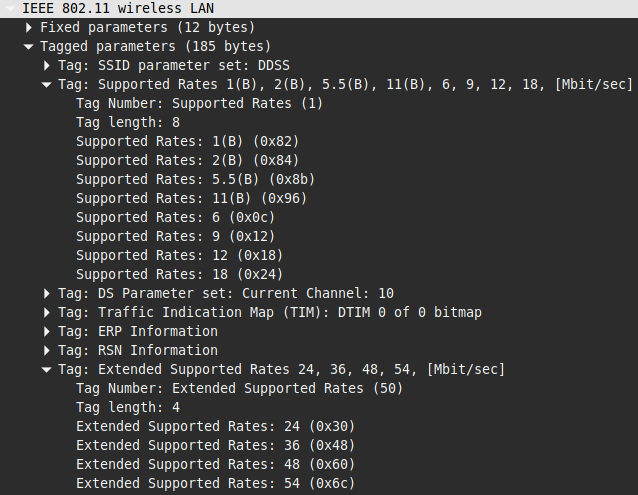
\includegraphics[width=1\linewidth]{./imagens/ex3_debito_max.png}
  \end{subfigure}%
  \caption{Comparação do débito da trama com o máximo permitido na norma 802.11g.}
  \label{fig:debito_733}
\end{figure}


\clearpage

\section{Scanning Passivo e Scanning Ativo}
\subsection{Exercício 4}
\subsubsection{Questão}\rule[-10pt]{0pt}{10pt}\\

Selecione uma trama beacon (cujo número de ordem inclua o seu número de grupo [33]). Esta trama pertence a que tipo de tramas 802.11? Indique o valor dos seus identificadores de tipo e de subtipo. Em que parte concreta do cabeçalho da trama estão especificados (ver anexo)?

\subsubsection{Resposta}\rule[-10pt]{0pt}{10pt}\\

[Trama nº 233]
Esta trama é uma \textit{Management Frame} (identificador 00) de subtipo \textit{Beacon} (identificador 1000 em binário, 8 em decimal). Os identificadores estão presentes em IEEE 802.11 Beacon Frame, no campo Frame Control, nos bits 4-5 e 0-3, respetivamente.

\subsubsection{Realização}\rule[-10pt]{0pt}{10pt}\\

\begin{figure}
  \begin{center}
  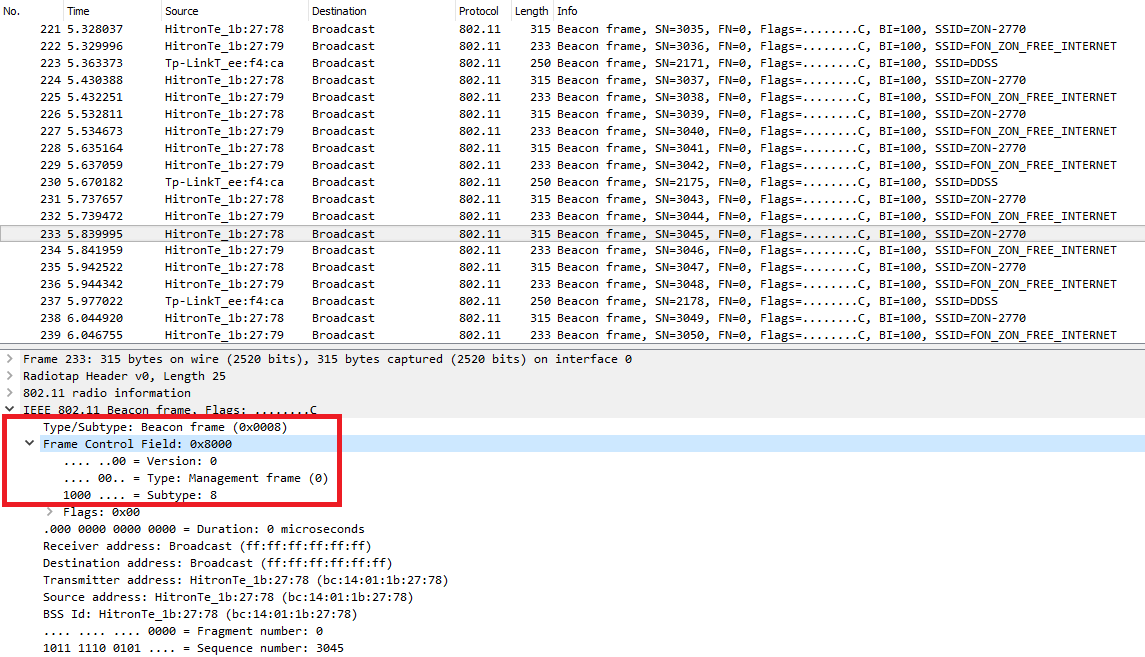
\includegraphics[scale=0.40]{imagens/tipo_subtipo.png} 
  \end{center}
  \caption{Os identificadores do tipo e subtipo da trama \textit{Beacon}.}
  \label{fig:type_field}
\end{figure} 

\clearpage
\subsection{Exercício 5}
\subsubsection{Questão}\rule[-10pt]{0pt}{10pt}\\

Liste todos os SSIDs dos APs (Access Points) que estão a operar na vizinhança da STA de captura? Explicite o modo como obteve essa informação. Como sugestão pode construir um filtro de visualização apropriado (tomando como base a resposta da alínea anterior) que lhe permita obter a listagem pretendida.

\subsubsection{Resposta}\rule[-10pt]{0pt}{10pt}\\

Ao aplicar o filtro \texttt{wlan.fc == 0x8000} , obtêm-se todas as tramas \textit{beacon} enviadas pelos AP's cirundantes. Observando o campo IEEE 802.11 wireless LAN -> Tagged parameters -> Tag: SSID parameter set -> SSID ao longo das tramas capturadas, determina-se que existem 3 AP's, com os SSID's ZON-2770, FON\_ZON\_FREE\_INTERNET e DDSS.

\subsubsection{Realização}\rule[-10pt]{0pt}{10pt}\\

\begin{figure}
  \begin{center}
  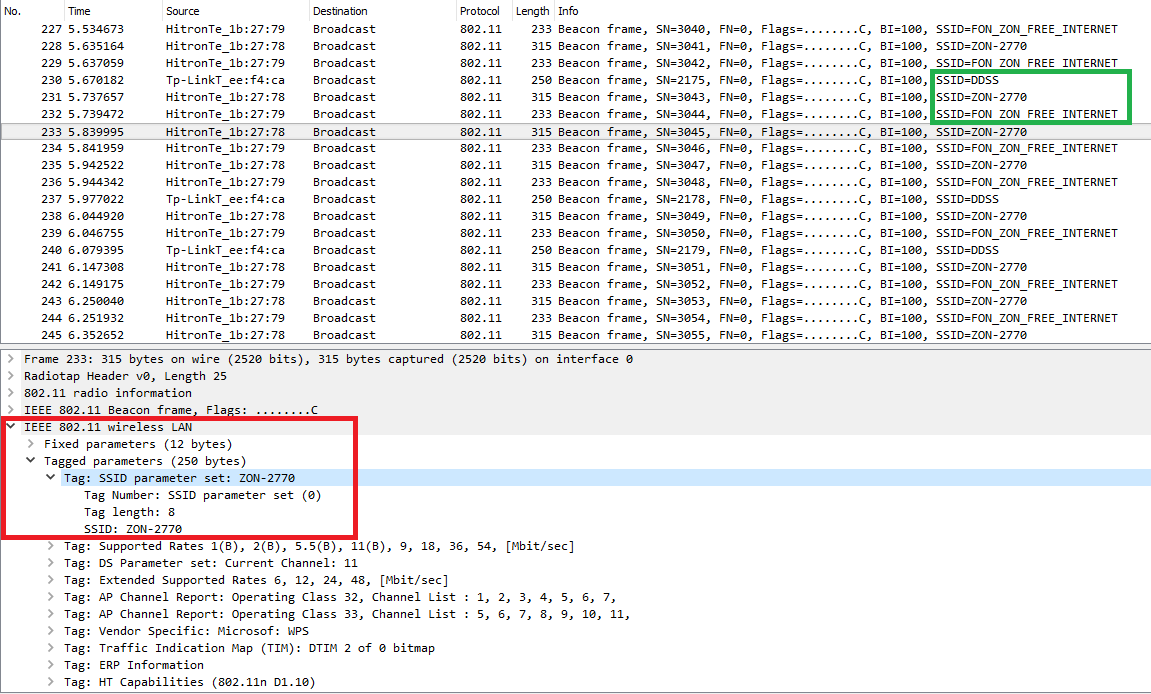
\includegraphics[scale=0.40]{imagens/SSID.png} 
  \end{center}
  \caption{O SSID da trama 233; O \textit{Wireshark} destaca esta informação por defeito.}
  \label{fig:ssid_field}
\end{figure}

\clearpage
\subsection{Exercício 6}
\subsubsection{Questão}\rule[-10pt]{0pt}{10pt}\\

Verifique se está a ser usado o método de detecção de erros (CRC), e se todas as tramas Beacon são recebidas corretamente. Justifique a conveniência em usar detecção de erros neste tipo de redes locais.

\subsubsection{Resposta}\rule[-10pt]{0pt}{10pt}\\

Está de facto a ser utilizada CRC, nomeadamente através de frame check sequence (FCS). Nem todas as tramas beacon estão a ser recebidas corretamente, visto que é possível encontrar uma pequena percentagem de tramas com um FCS incorreto.
É conveniente utilizar deteção de erros em redes sem fios visto que estes são por natureza dispostos a ter mais ruído do que os meios com fios, o que leva a uma maior probabilidade de corrupção de dados enviados. Deste modo, assegura-se que não ocorrem falhas de interpretação de informação ou desperdício de recursos.

\subsubsection{Realização}\rule[-10pt]{0pt}{10pt}\\

\begin{figure}
  \begin{center}
  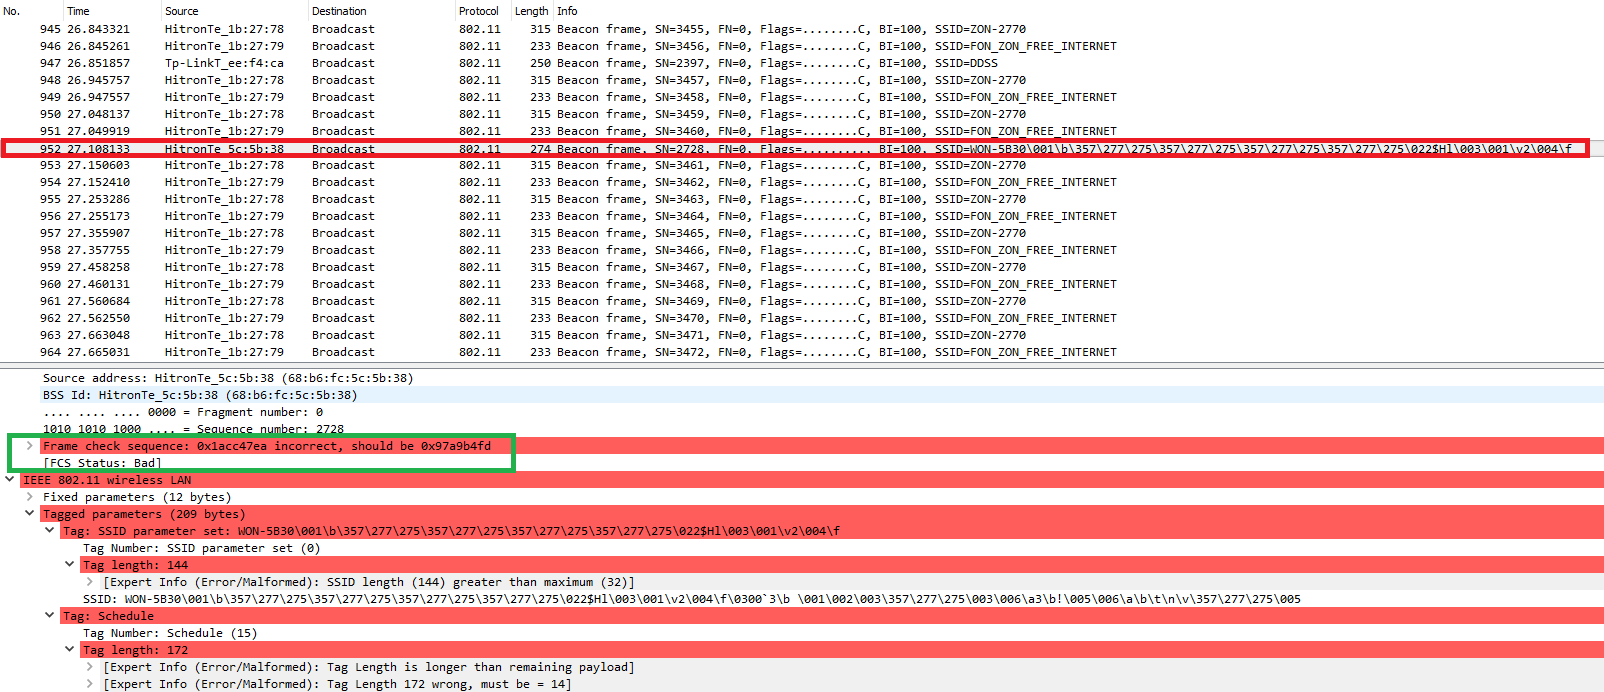
\includegraphics[scale=0.35]{imagens/FCS.png} 
  \end{center}
  \caption{O campo FCS de uma trama corrompida; nota-se que o \textit{Wireshark} destaca os campos corrompidos.}
  \label{fig:fcs_field}
\end{figure}

\clearpage
\subsection{Exercício 7}
\subsubsection{Questão}\rule[-10pt]{0pt}{10pt}\\

Para dois dos APs identificados, indique qual é o intervalo de tempo previsto entre tramas beacon consecutivas? (Nota: este valor é anunciado na própria trama beacon). Na prática, a periodicidade de tramas beacon é verificada? Tente explicar porquê.

\subsubsection{Resposta}\rule[-10pt]{0pt}{10pt}\\

SSID ZON-2770: intervalo de acordo com a trama: 0.102400 s

SSID FON\_ZON\_FREE\_INTERNET: intervalo de acordo com a trama: 0.102400 s

Na prática, o valor do intervalo de tempo varia cerca de $ \pm $ 0.0001 s relativamente ao intervalo previsto. Isto pode se dever ao facto de que é necessário fazer deteção de erros ao receber cada trama. Isto é tido em conta pelo beacon interval e, como o tempo necessário para fazer a verificação é imutável, ocorrem pequenas variâncias no intervalo entre tramas.

\subsubsection{Realização}\rule[-10pt]{0pt}{10pt}\\

\begin{figure}
  \begin{center}
  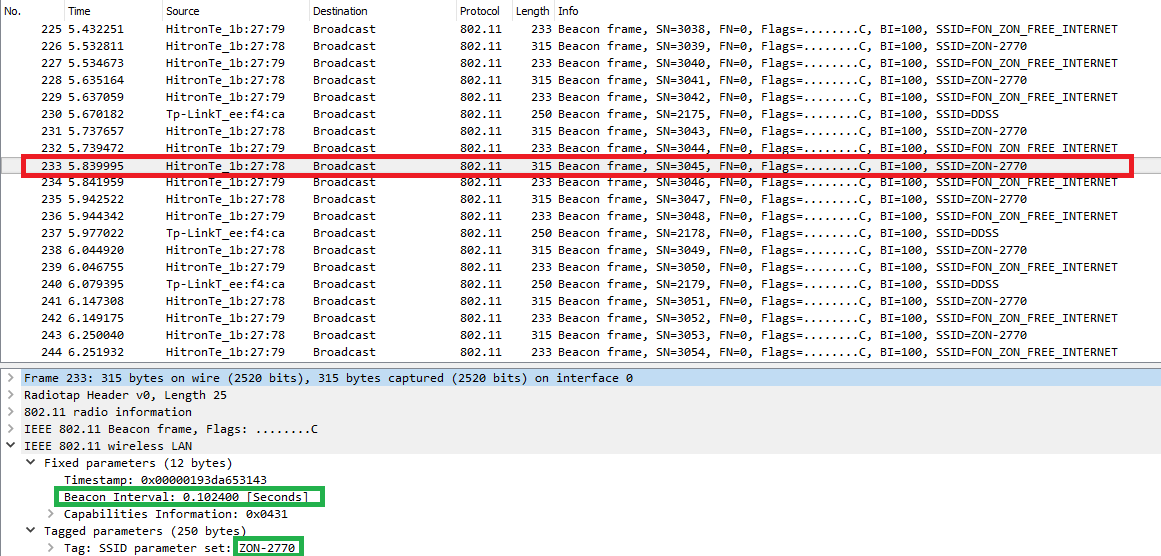
\includegraphics[scale=0.35]{imagens/ZON_BI.png} 
  \end{center}
  \caption{Um exemplo de um intervalo real entre duas tramas beacon do mesmo AP, igual a 0.102527 s.}
  \label{fig:zon_interval}
\end{figure}

\begin{figure}
  \begin{center}
  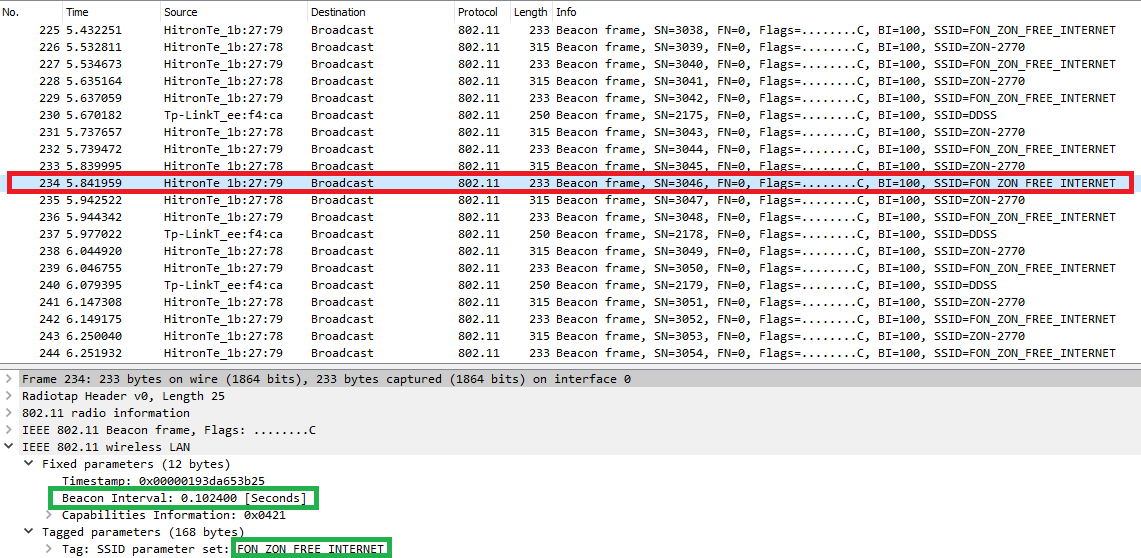
\includegraphics[scale=0.35]{imagens/FONZON_BI.png} 
  \end{center}
  \caption{Um exemplo de um intervalo real entre duas tramas beacon do mesmo AP, igual a 0.102383 s.}
  \label{fig:zon_interval}
\end{figure}


\clearpage
\subsection{Exercício 8}
\subsubsection{Questão}\rule[-10pt]{0pt}{10pt}\\

Identifique e registe todos os endereços MAC usados nas tramas beacon enviadas pelos APs. Recorde que o endereçamento está definido no cabeçalho das tramas 802.11, podendo ser utilizados até quatro endereços com diferente semântica. Para uma descrição detalhada da estrutura da trama 802.11, consulte o anexo ao enunciado.

\subsubsection{Resposta}\rule[-10pt]{0pt}{10pt}\\



\subsubsection{Realização}\rule[-10pt]{0pt}{10pt}\\



\clearpage
\subsection{Exercício 9}
\subsubsection{Questão}\rule[-10pt]{0pt}{10pt}\\

As tramas beacon anunciam que o AP pode suportar vários débitos de base assim como vários “extended supported rates”. Indique quais são esses débitos?

\subsubsection{Resposta}\rule[-10pt]{0pt}{10pt}\\



\subsubsection{Realização}\rule[-10pt]{0pt}{10pt}\\



\clearpage
\subsection{Exercício 10}
\subsubsection{Questão}\rule[-10pt]{0pt}{10pt}\\

Estabeleça um filtro Wireshark apropriado que lhe permita visualizar todas as tramas probing request ou probing response, simultaneamente.

\subsubsection{Resposta}\rule[-10pt]{0pt}{10pt}\\



\subsubsection{Realização}\rule[-10pt]{0pt}{10pt}\\




\clearpage
\subsection{Exercício 11}
\subsubsection{Questão}\rule[-10pt]{0pt}{10pt}\\

Identifique um probing request para o qual tenha havido um probing response. Face ao endereçamento usado, indique a que sistemas são endereçadas estas tramas e explique qual o propósito das mesmas?

\subsubsection{Resposta}\rule[-10pt]{0pt}{10pt}\\



\subsubsection{Realização}\rule[-10pt]{0pt}{10pt}\\



\clearpage

\section{Processo de Associação}
\subsection{Exercício 12}
\subsubsection{Questão}\rule[-10pt]{0pt}{10pt}\\

Identifique uma sequência de tramas que corresponda a um processo de associação completo entre a STA e o AP, incluindo a fase de autenticação.

\subsubsection{Resposta}\rule[-10pt]{0pt}{10pt}\\

Uma possível sequência de tramas que correspondem a um processo de associação completo são as identificadas pelos números 2027 (autenticação STA -> AP), 2029 (autenticação AP -> STA), 2031 (pedido de associação) e 2035 (resposta ao pedido de associação). Além destas é possível identificar tramas de confirmação de receção (\textit{Acknowlegment}) entre todas as tramas trocadas entre o STA e o AP.

\subsubsection{Realização}\rule[-10pt]{0pt}{10pt}\\

\begin{figure}
  \begin{center}
  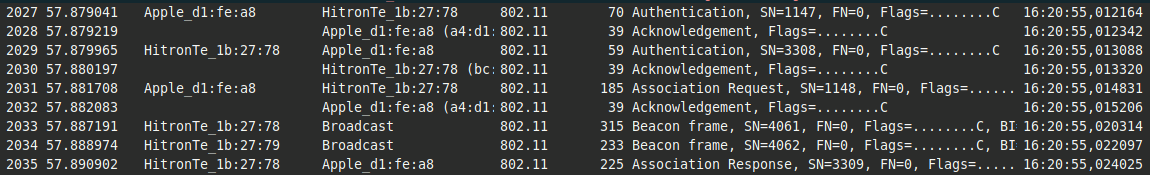
\includegraphics[scale=0.35]{./imagens/assoc_seq.png} 
  \end{center}
  \caption{Sequência de tramas trocadas no processo de associação.}
  \label{fig:assoc_seq}
\end{figure}


\clearpage
\subsection{Exercício 13}
\subsubsection{Questão}\rule[-10pt]{0pt}{10pt}\\

Efetue um diagrama que ilustre a sequência de todas as tramas trocadas no processo.

\subsubsection{Resposta}\rule[-10pt]{0pt}{10pt}\\

\begin{figure}
  \begin{center}
  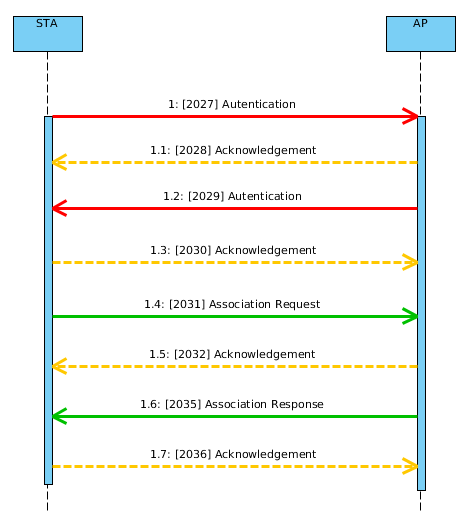
\includegraphics[scale=0.6]{./imagens/diag_assoc_seq.png} 
  \end{center}
  \caption{Diagrama da sequência de tramas trocadas no processo de associação, realizado no \textit{Visual Paradigm}.}
  \label{fig:diag_assoc_seq}
\end{figure}

\subsubsection{Realização}\rule[-10pt]{0pt}{10pt}\\



\clearpage

\section{Transferência de Dados}
\subsection{Exercício 14}
\subsubsection{Questão}\rule[-10pt]{0pt}{10pt}\\

Considere a trama de dados nº1054. Sabendo que o campo Frame Control contido no cabeçalho das tramas 802.11 permite especificar a direccionalidade das tramas, o que pode concluir face à direccionalidade dessa trama, será local à WLAN?

\subsubsection{Resposta}\rule[-10pt]{0pt}{10pt}\\


\subsubsection{Realização}\rule[-10pt]{0pt}{10pt}\\


\clearpage
\subsection{Exercício 15}
\subsubsection{Questão}\rule[-10pt]{0pt}{10pt}\\

Para a trama de dados nº1054, transcreva os endereços MAC em uso, identificando qual o endereço MAC correspondente ao host sem fios (STA), ao AP e ao router de acesso ao sistema de distribuição?

\subsubsection{Resposta}\rule[-10pt]{0pt}{10pt}\\



\subsubsection{Realização}\rule[-10pt]{0pt}{10pt}\\



\clearpage
\subsection{Exercício 16}
\subsubsection{Questão}\rule[-10pt]{0pt}{10pt}\\

Como interpreta a trama nº1060 face à sua direccionalidade e endereçamento MAC?

\subsubsection{Resposta}\rule[-10pt]{0pt}{10pt}\\



\subsubsection{Realização}\rule[-10pt]{0pt}{10pt}\\



\clearpage
\subsection{Exercício 17}
\subsubsection{Questão}\rule[-10pt]{0pt}{10pt}\\

Que subtipo de tramas de controlo são transmitidas ao longo da transferência de dados acima mencionada? Tente explicar porque razão têm de existir (contrariamente ao que acontece numa rede Ethernet.)

\subsubsection{Resposta}\rule[-10pt]{0pt}{10pt}\\



\subsubsection{Realização}\rule[-10pt]{0pt}{10pt}\\



\clearpage
\subsection{Exercício 18}
\subsubsection{Questão}\rule[-10pt]{0pt}{10pt}\\

O uso de tramas Request To Send e Clear To Send, apesar de opcional, é comum para efetuar "pré-reserva" do acesso ao meio quando se pretende enviar tramas de dados, com o intuito de reduzir o número de colisões resultante maioritariamente de STAs escondidas. Para o exemplo acima, verifique se está a ser usada a opção RTS/CTS na troca de dados entre a STA e o AP/Router da WLAN, identificando a direccionalidade das tramas e os sistemas envolvidos.

\subsubsection{Resposta}\rule[-10pt]{0pt}{10pt}\\



\subsubsection{Realização}\rule[-10pt]{0pt}{10pt}\\



\clearpage

\section{Conclusões}

\hspace{5mm} Neste trabalho foi abordada a camada de ligação lógica da pilha OSI e alguns dos seus componentes. 

Primeiramente, procedeu-se à compreensão das tramas \textit{ethernet} que permitiu consolidar bases para analisar as mensagens de ARP e as suas características. A compreensão do protocolo ARP, auxiliada pelos exercícios propostos, permitiu perceber a área em que este protocolo atua e quais as suas consequências.

Por fim, percebeu-se o impacto que têm os diferentes sistemas que constituem a rede. Nomeadamente, o domínio de colisão depende em grande parte da topologia utilizada e caso esta não previna antecipadamente as colisões de tramas na rede, são então utilizados protocolos que tem como objetivo evitar essas mesmas colisões através de diferentes abordagens, como é o caso do protocolo CSMA/CD que apenas transmite quando a rede se encontra desocupada.

%BIBLIOGRAFIA
\bibliographystyle{splncs}
\bibliography{ficheirodebibliografia}

\end{document}
